%----------------------------------------------------------------------------------------
%	PACKAGES AND DOCUMENT CONFIGURATIONS
%----------------------------------------------------------------------------------------

\documentclass[12pt]{article}

\usepackage[english]{babel}
\usepackage[utf8]{inputenc}
\usepackage[T1]{fontenc}
\usepackage[top=2cm, bottom=2cm, left=3cm, right=3cm]{geometry}
\usepackage{graphicx}
\usepackage[babel=true]{csquotes} % csquotes va utiliser la langue définie dans babel

\setlength\parindent{0pt} % Removes all indentation from paragraphs

\begin{document}

\textsc{École Polytechnique (X)} \\
\textsc{Research Internship} \\

\vspace*{\fill}
\begin{center}
\begin{large}
\textsc{Documentation} \\
\textsl{LifeBand : The App} \\
\end{large}
\end{center}
\vspace*{\fill}

\begin{tabular}{l r}
Author : & Louis Faucon \\
Email : & lpfaucon@gmail.com \\
Date : & \today \\
\end{tabular}
\newpage



%----------------------------------------------------------------------------------------
%	ABSTRACT
%----------------------------------------------------------------------------------------
\section*{Introduction}
\paragraph{} LifeBand is an app ... 

\paragraph{} This document contains... 


\end{abstract}
\newpage

%----------------------------------------------------------------------------------------
% SOMMAIRE
%----------------------------------------------------------------------------------------
\tableofcontents

%----------------------------------------------------------------------------------------
%	SECTION
%----------------------------------------------------------------------------------------
\newpage
\section{Architecture Overview}
%----------------------------------------------------------------------------------------
\subsection{Activities}
\paragraph{}An \verb?Activity? object implements the functions of the screen the user interacts with. It uses an xml file from \verb?res/layout/? to describe its layout. The diagram (Fig. \ref{fig:activity} shows how user can navigate from one to another.

\begin{description}
\item[- MainActivity] is the main activity. You can see the two bands and access other activities.
\item[- ColorActivity] is the nudges sending activity. You can choose between ten colours and then click on SEND.
\item[- SettingsActivity] is for setting up user information. You just need to fill in name and login and then click on SAVE.
\item[- SettingsLocationActivity] is for setting up location information. You need to click on the buttons once when at home and once when at work.
\end{description}


\begin{figure}[ht]
	\centering
		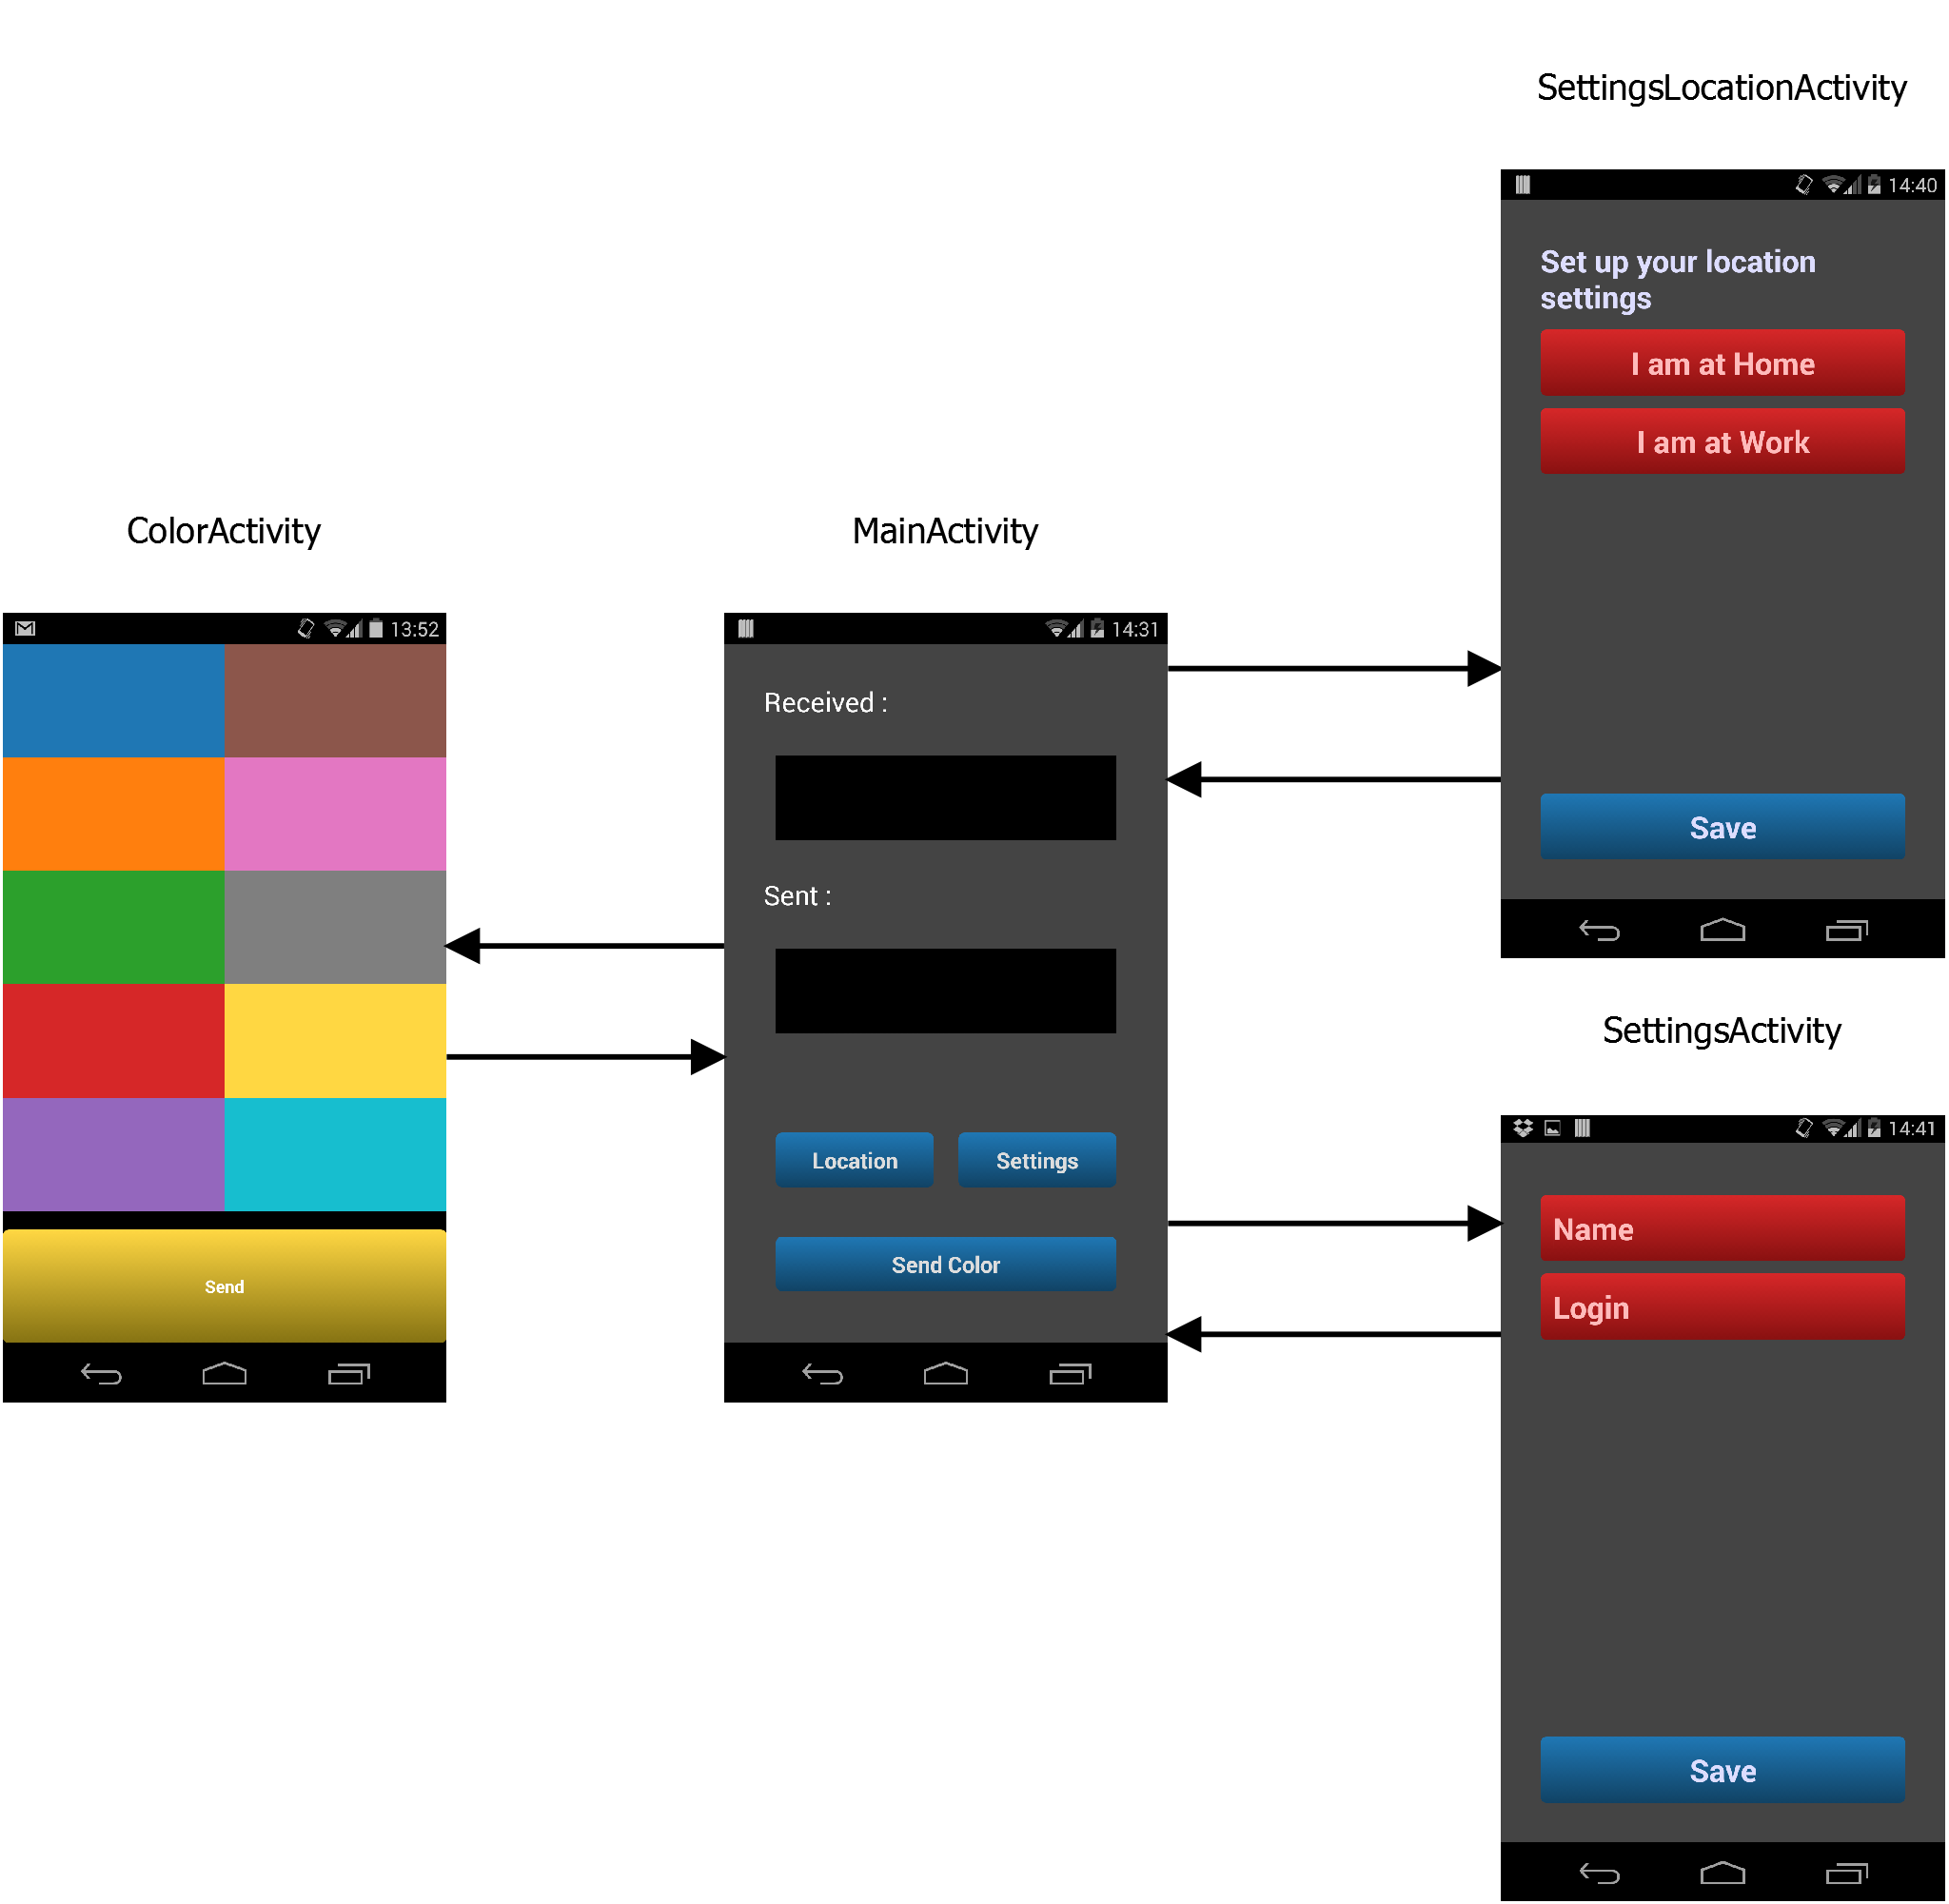
\includegraphics[width=12cm]{graphs/activity.png}
	\caption{Activities architecture}
	\label{fig:activity}
\end{figure}

%----------------------------------------------------------------------------------------
\subsection{Location updates}
\paragraph{}The following diagram (Fig. \ref{fig:locationupdates}) shows the passive process of sending locations updates.

\begin{figure}[ht]
	\centering
		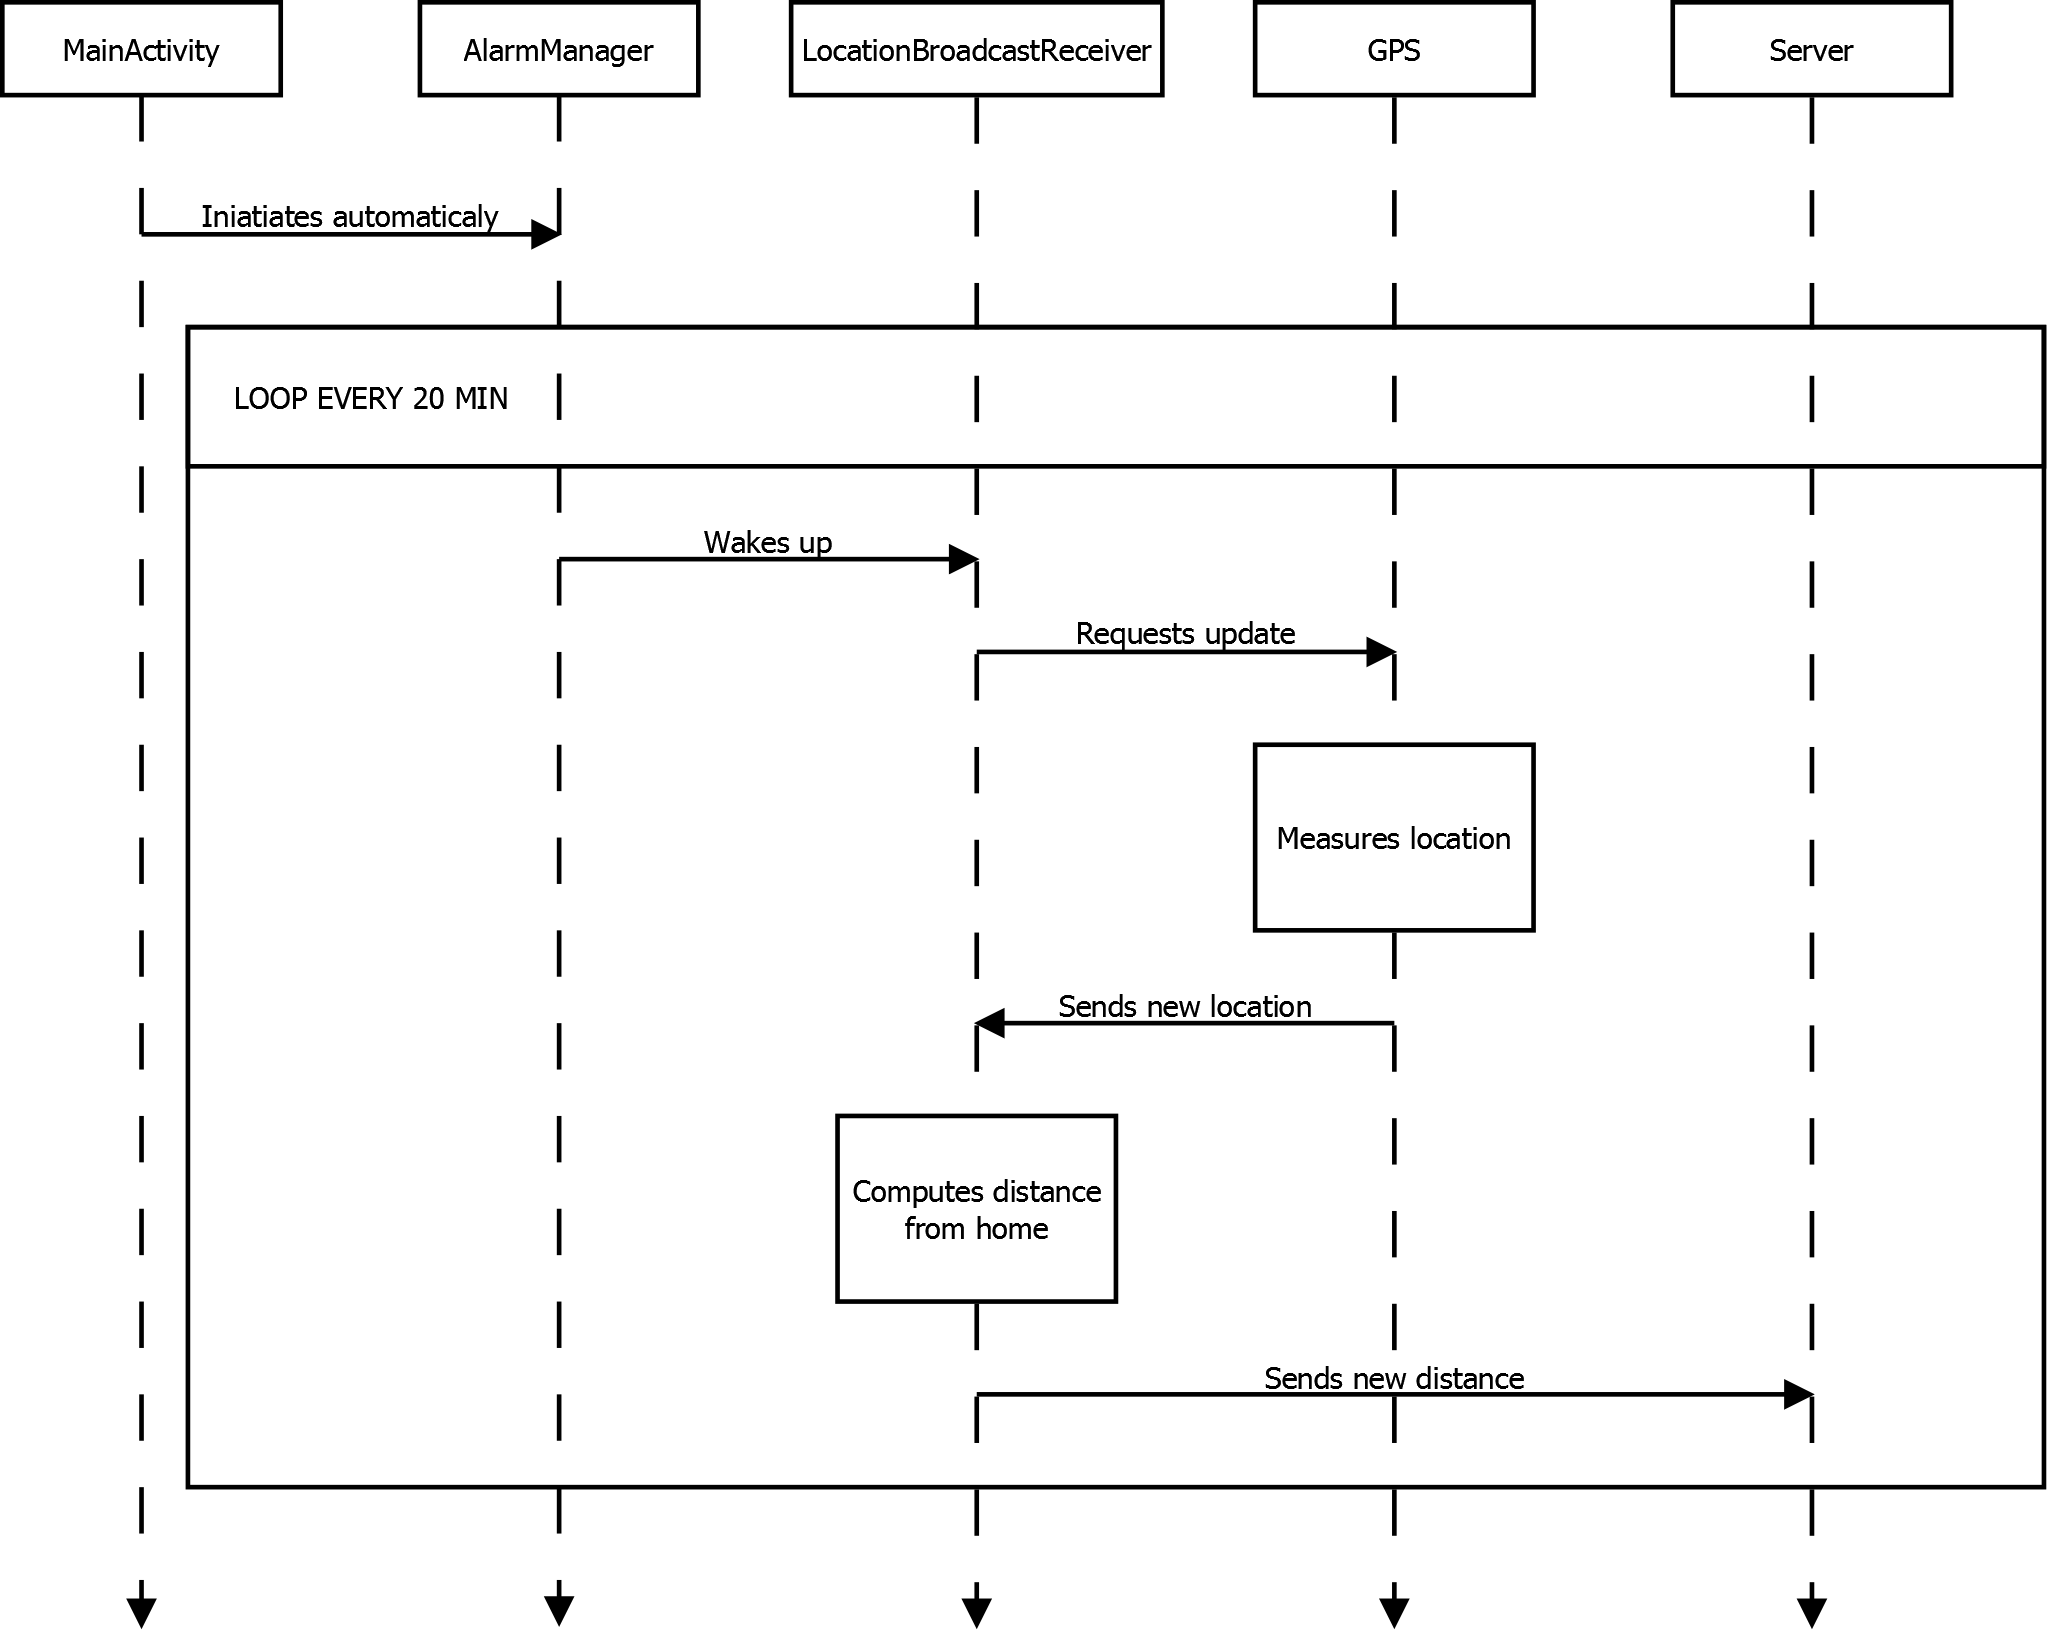
\includegraphics[width=16cm]{graphs/locationupdates.png}
	\caption{Location updates}
	\label{fig:locationupdates}
\end{figure}


%----------------------------------------------------------------------------------------
\subsection{Saving data}
%----------------------------------------------------------------------------------------
\subsubsection{Preferences}
\paragraph{}The \verb?Preferences? are good for saving small static amount of data for the application. The code for using \verb?Preferences? is in the \verb?class SettingsUtils?.
\paragraph{}
\begin{tabular}{rl}
	\verb?String name? & User's name \\
	\verb?String login? & Login to link two partners \\
	\verb?String regid? & ID for google cloud messaging \\
	\verb?String bffid? & Partner's ID for google cloud messaging\\
	\verb?float home_lat? & Latitude of home place \\
	\verb?float home_lon? & Longitude of home place \\
	\verb?float work_lat? & Latitude of work place \\
	\verb?float work_lon? & Longitude of work place \\
\end{tabular}

%----------------------------------------------------------------------------------------
\subsubsection{SQL database}
\paragraph{}The \verb?SQL database? is good for saving larger amount of data that often change.





%----------------------------------------------------------------------------------------
\subsection{Messages}
%----------------------------------------------------------------------------------------
\subsubsection{Messages from the app}
\paragraph{}The app sends messages to the server using POST end GET requests. This is done by a static method of \verb?LinkToServerManager?.
\paragraph{}
\begin{tabular}{l|l|l|l|l}
type & time & message & from & to \\
\hline
\hline
\verb?colortoken? & \verb?long? & an \verb?int? for the color & \verb?String regid? & \verb?String bffid? \\
\verb?locationtoken? & \verb?long? & an \verb?int? for the distance & \verb?String regid? & \verb?String bffid? \\
\end{tabular}



%----------------------------------------------------------------------------------------
\subsubsection{Messages from the server}

\paragraph{}The server sends messages to the phones using \textsc{google cloud messaging}. Every time a message is received from the app, the server send two messages, one to the sender with type \verb?sent? and one to his partner with type \verb?received?.
\paragraph{}
\begin{tabular}{l|l|l}
type & time & message \\
\hline
\hline
\verb?colortokensent? & \verb?long? & an \verb?int? for the color \\
\verb?colortokenreceived? & \verb?long? & an \verb?int? for the color \\
\verb?locationtokensent? & \verb?long? & an \verb?int? for the distance \\
\verb?locationtokenreceived? & \verb?long? & an \verb?int? for the distance \\
\end{tabular}


%----------------------------------------------------------------------------------------
\subsubsection{Special messages for registration}
\paragraph{}The first message is sent from the phone and contains the \verb?name?, the \verb?login? and the \verb?regid?. Then the server sends two messages : the first one to acknowledge the registration and the second one containing the partner's id.


%----------------------------------------------------------------------------------------
\newpage
\subsection{General}

\begin{figure}[ht]
	\centering
		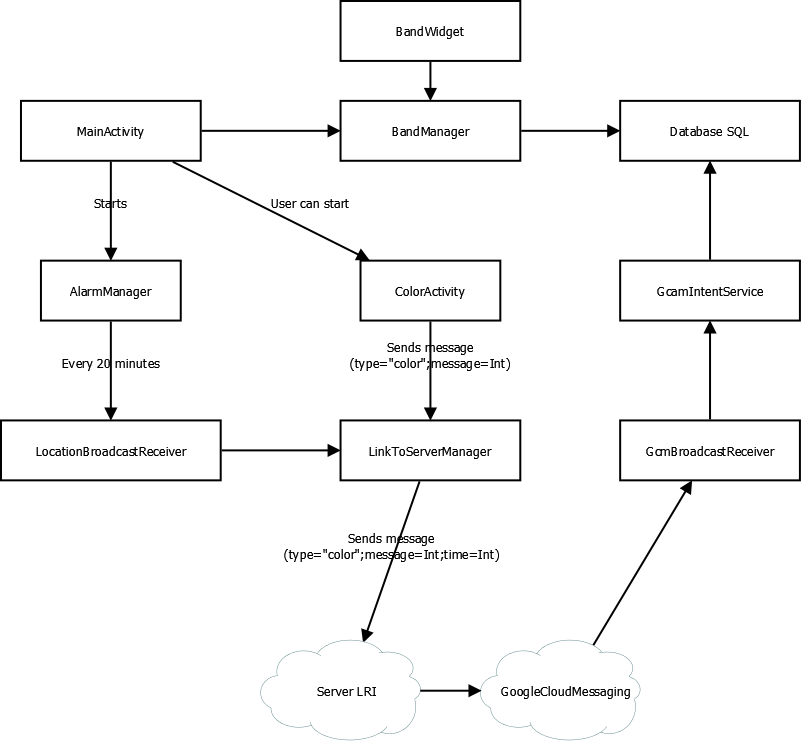
\includegraphics[width=16cm]{graphs/global.png}
	\caption{General architecture}
	\label{fig:global}
\end{figure}

%----------------------------------------------------------------------------------------
%	SECTION
%----------------------------------------------------------------------------------------
\newpage
\section{Complete Documentation}
%----------------------------------------------------------------------------------------
\subsection{lri.prototype.cosquare.app.bff}
%----------------------------------------------------------------------------------------
\subsubsection{BandManager}
\paragraph{}The two methods \verb?getBitmapReceived? and \verb?getBitmapSent? give the band bitmap images (See Figure \ref{fig:band}). The band can be configuered by changing the values of \verb?LENGTH_TIMELINE?, \verb?LENGTH_UNIT?, \verb?WIDTH_BITMAP? and \verb?HEIGHT_BITMAP?.

\begin{figure}[ht]
	\centering
		
\includegraphics[width=8cm]{pictures/band.png}
	\caption{Example of the output bitmap.}
	\label{fig:band}
\end{figure}

\begin{verbatim}
private static final int LENGTH_TIMELINE = 10 * HOUR;
private static final int LENGTH_UNIT = HOUR;
private static final int WIDTH_BITMAP = 1024;
private static final int HEIGHT_BITMAP = 256;

public static Bitmap getBitmapReceived(Context context){...}
public static Bitmap getBitmapSent(Context context){...}
\end{verbatim}

%----------------------------------------------------------------------------------------
\subsubsection{ColorActivity}
\paragraph{}\verb?ColorActivity? uses the layout \verb?res/layout/activity_color.xml? (See Figure \ref{fig:color}). The activity shows 10 buttons whose color are described in the file \verb?res/values/colors.xml?. The method \verb?onClick? selects a color and the method \verb?send? sends it.

\begin{figure}[ht]
	\centering
		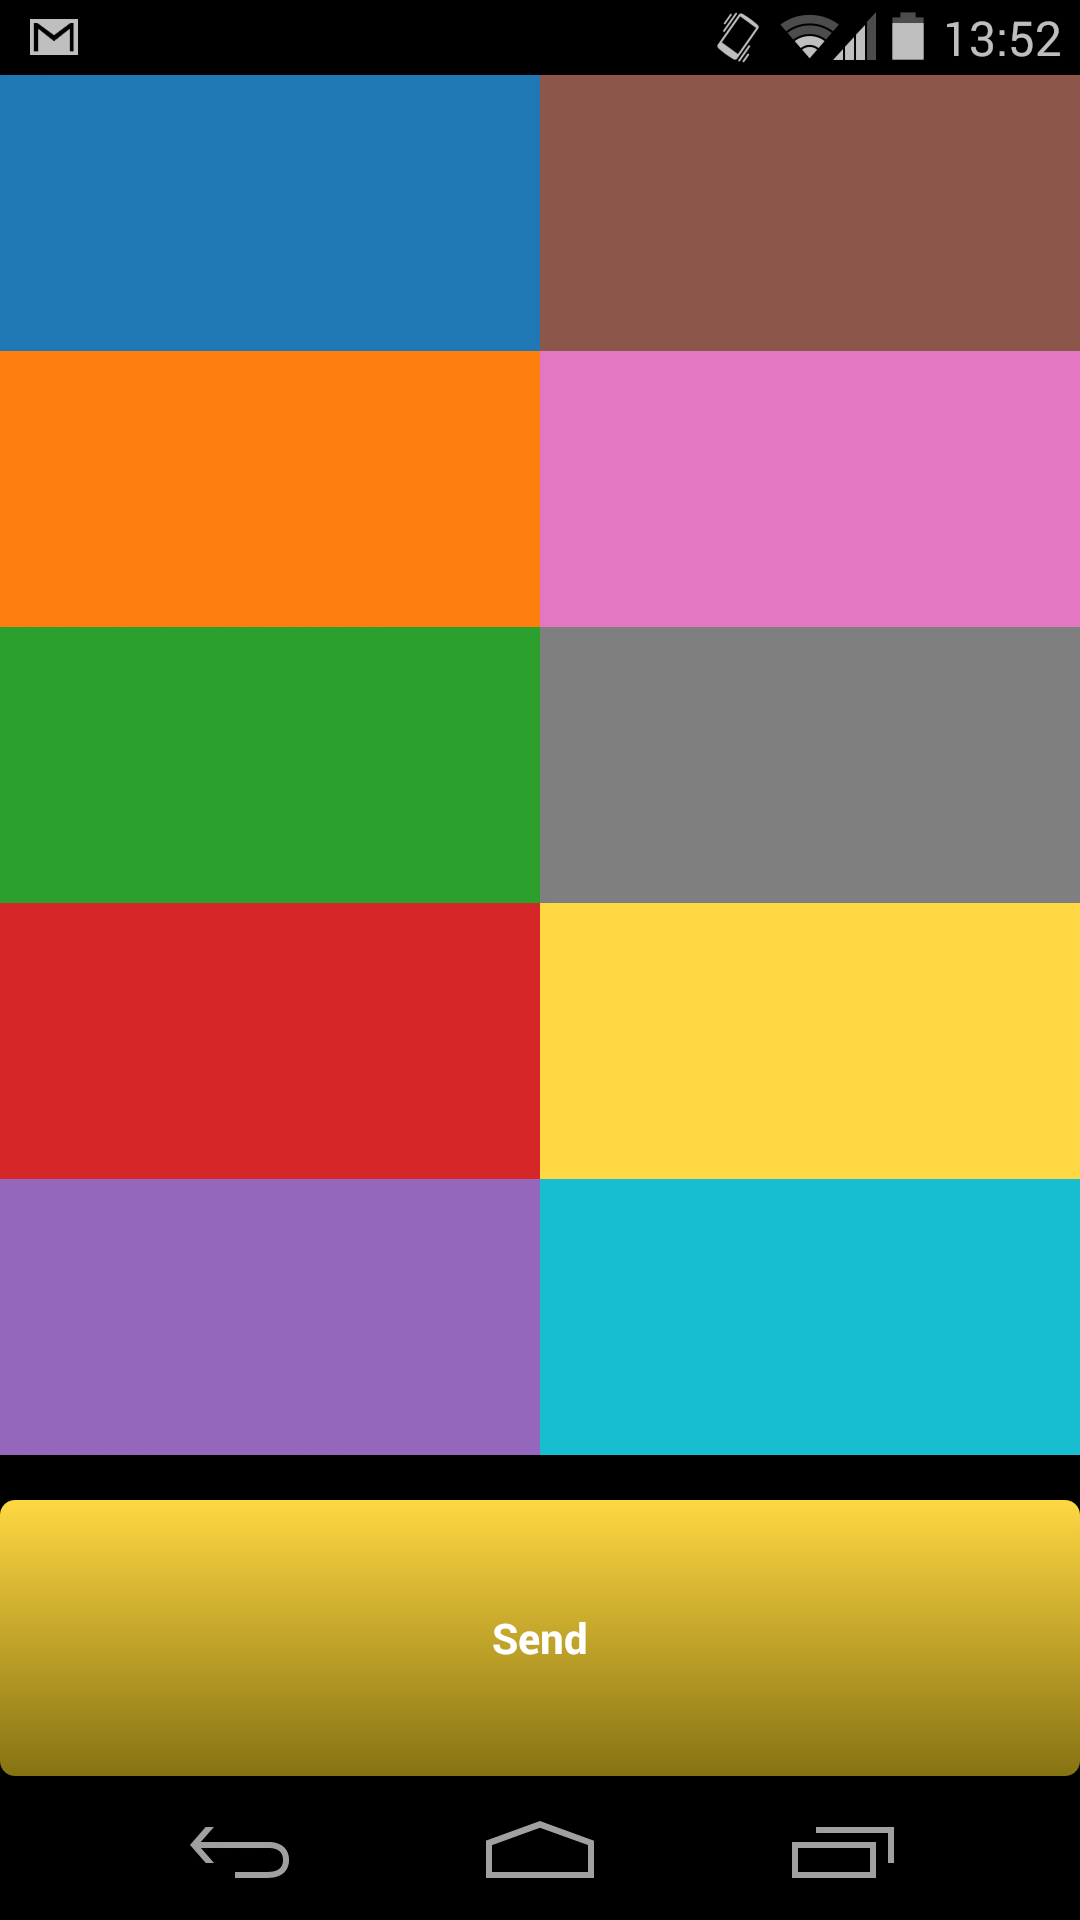
\includegraphics[width=4cm]{pictures/color.png}
	\caption{ColorActivity layout}
	\label{fig:color}
\end{figure}

\begin{verbatim}
public void onClick(View view){...}
public void send(View view){...}
\end{verbatim}
%----------------------------------------------------------------------------------------
\subsubsection{ColorManager}
\paragraph{}This class has only one static method \verb?getColor?. It takes two arguments an \verb?int p? between 0 and 100 and a color and outputs a new color darker or lighter depending on \verb?p?. The output color is the same as the input for \verb?p=?50

\begin{figure}[ht]
	\centering
		
\includegraphics[width=8cm]{pictures/scale.png}
	\caption{Color output for purple and p=0 on the left to p=100 on the right}
	\label{fig:scale}
\end{figure}

\begin{verbatim}
public static int getColor(int p,int color){...}
\end{verbatim}
%----------------------------------------------------------------------------------------
\subsection{lri.prototype.cosquare.app.gcm}
%----------------------------------------------------------------------------------------
\subsubsection{GcmBroadcastReceiver}
\paragraph{}This class is an always on receiver that listen to the \textsc{Google Cloud Messaging}. When a message is received the receiver just gives it to \verb?GcmIntentService?.


%----------------------------------------------------------------------------------------
\subsubsection{GcmIntentService}
\paragraph{}This service handles the messages from the server. The messages contain three fields \verb?type?, \verb?time? and \verb?message?.

%----------------------------------------------------------------------------------------
\subsubsection{GcmManager}
\paragraph{}This class is just used at the first launch of the app to register an ID with the \textsc{Google Clood Messagging}. The \verb?SENDER_ID? is the ID of the server that sends messages. It is linked with the google account of the developer.

\begin{verbatim}
String SENDER_ID = "403235248512";
public void register(){...}
\end{verbatim}


%----------------------------------------------------------------------------------------
\subsection{lri.prototype.cosquare.app.location}
%----------------------------------------------------------------------------------------
\subsubsection{LocationBroadcastReceiver}
\paragraph{} \verb?LocationBroadcastReceiver? is an always on receiver that receives messages every 20 minutes from an \verb?AlarmManager? and wakes up the GPS to measure location and send it.


%----------------------------------------------------------------------------------------
\subsubsection{LocationUtils}
\paragraph{}\verb?TIME_BETWEEN_UPDATES? is used to configured the \verb?AlarmManager? that ask for location updates. The two other methods are just useful. 

\begin{verbatim}
static public int TIME_BETWEEN_UPDATES = 20*MINUTE;
static public float distanceFromHomeToWork(Context context){...}
static public float distanceFromHome(Context context,Location location){...}
\end{verbatim}

%----------------------------------------------------------------------------------------
\subsection{lri.prototype.cosquare.app.server}
%----------------------------------------------------------------------------------------
\subsubsection{LinkToServerManager}
\paragraph{}This class has static methods to send messages to the server. 

\begin{verbatim}
static final String SERVER_URL = "https://www.lri.fr/~faucon/gcmserver.php?todo=";

public static void sendRegistrationInfo(String name,String login,Context c){...}
public static void sendLocationToken(Context c, final int distance){...}
public static void sendColorToken(Context c, final int color){...}
\end{verbatim}




%----------------------------------------------------------------------------------------
\subsection{lri.prototype.cosquare.app.settings}
%----------------------------------------------------------------------------------------
\subsubsection{SettingsActivity}
\paragraph{}\verb?SettingsActivity? uses the layout \verb?res/layout/activity_settings.xml? (See Figure \ref{fig:user}). The activity shows 2 \verb?EditText?s that must be filled in by a name and a login.

\begin{figure}[ht]
	\centering
		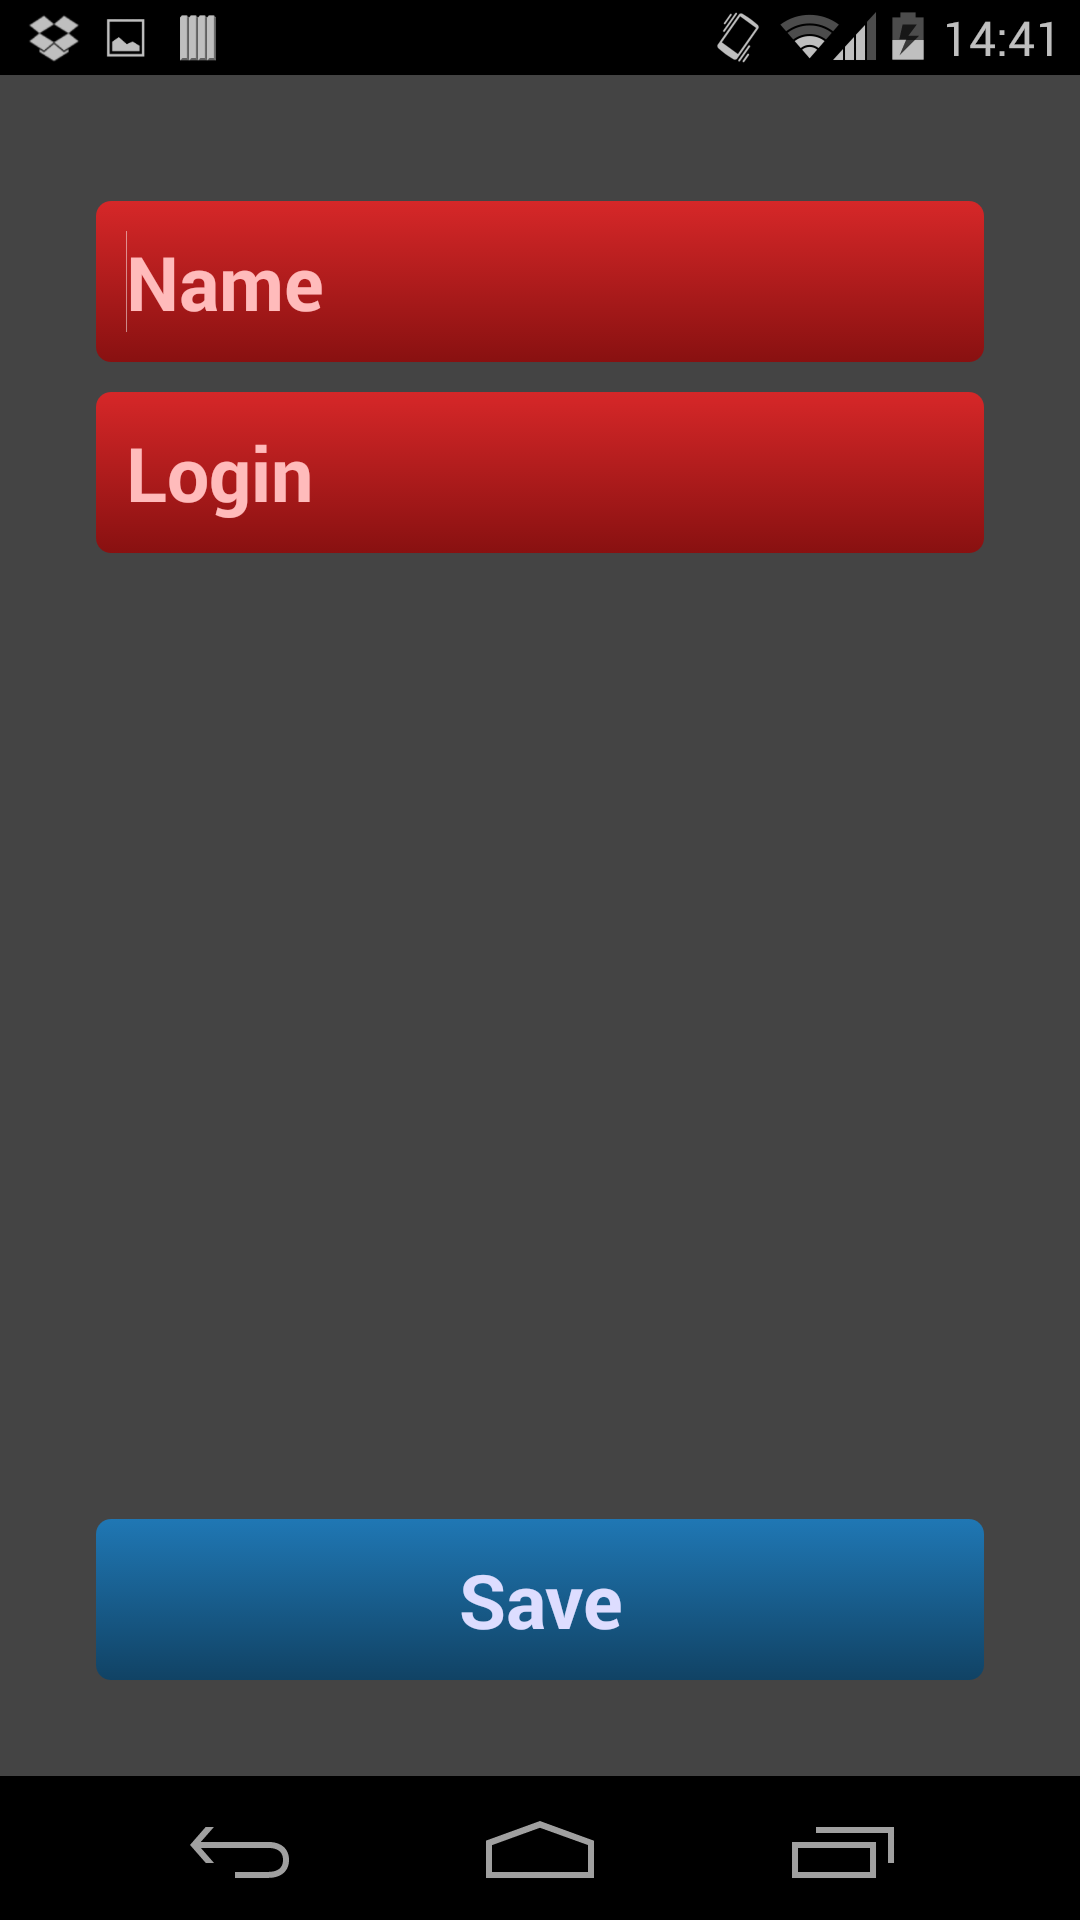
\includegraphics[width=4cm]{pictures/user.png}
	\caption{SettingsActivity layout}
	\label{fig:user}
\end{figure}

%----------------------------------------------------------------------------------------
\subsubsection{SettingsLocationActivity}
\paragraph{}\verb?SettingsLocationActivity? uses the layout \verb?res/layout/activity_settings.xml? (See Figure \ref{fig:location}). The activity shows 2 \verb?Button?s that, once clicked, register in the preferences the present location as Work or Home.

\begin{figure}[ht]
	\centering
		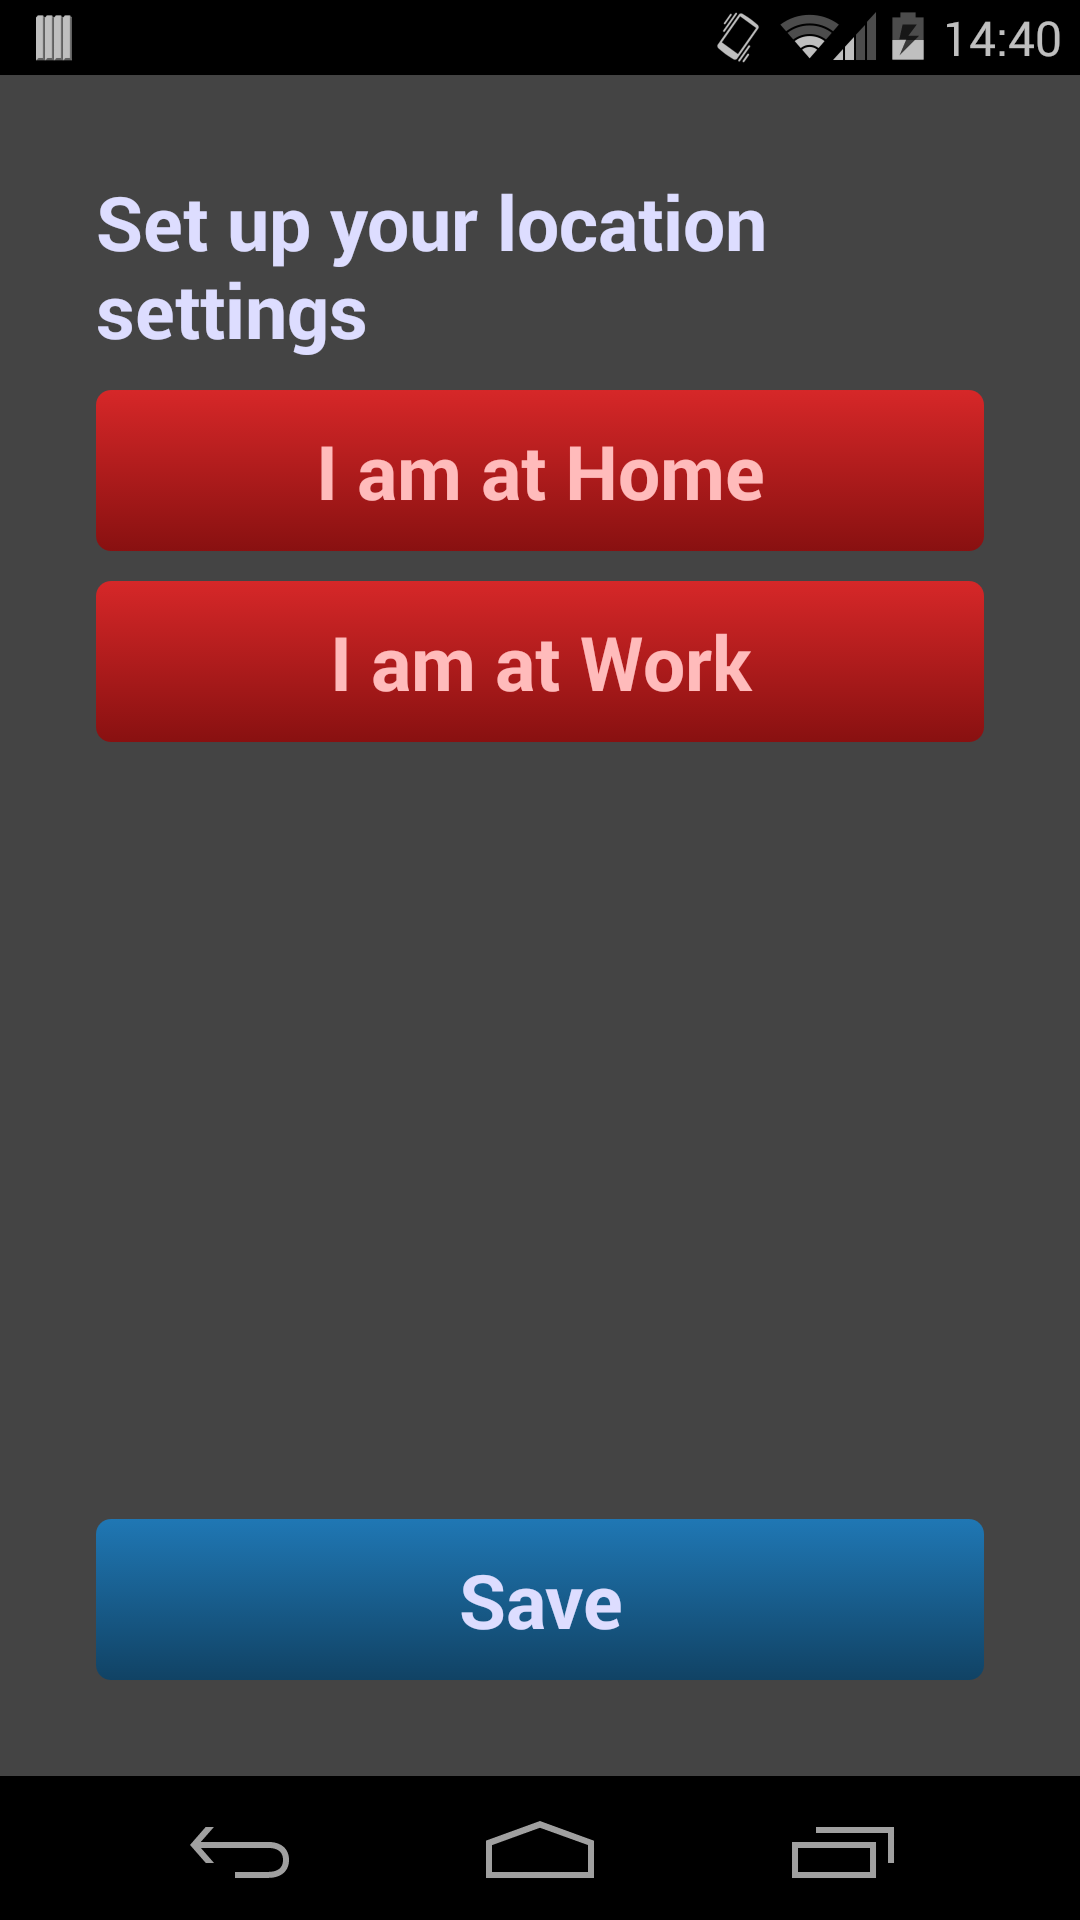
\includegraphics[width=4cm]{pictures/location.png}
	\caption{SettingsLocationActivity layout}
	\label{fig:location}
\end{figure}



%----------------------------------------------------------------------------------------
\subsubsection{SettingsLocationUtils}
\paragraph{}This class has useful static methods to record and retrieve information in the \verb?Preferences? of the application.

\begin{verbatim}
    //GETTERS
    public static String getName(Context context){...}
    public static String getLogin(Context context){...}
    public static String getRegid(Context context){...}
    public static String getBffid(Context context){...}
    public static Location getHome(Context context){...}
    public static Location getWork(Context context){...}

    //SETTERS
    public static void setUserInfo(String name,String login,Context context){...}
    public static void setRegid(String regid,Context context){...}
    public static void setBffid(String bffid,Context context){...}
    public static void setHome(Context c){...}
    public static void setWork(Context c){...}
\end{verbatim}


%----------------------------------------------------------------------------------------
\subsection{lri.prototype.cosquare.app.sqldatabase}
\paragraph{}The \verb?SQL databas? of the application contains four tables :
\verb?ColorTokenReceived?, \verb?ColorTokenSent?, \verb?LocationTokenReceived? and \verb?LocationTokenSent?. Each of this class has a method \verb?add? and a method \verb?getAll?. These are used when a message is received or when the app needs to display the band.

\paragraph{}\verb?DatabaseUtils? contains easier to use methods to add data in the database. \paragraph{}\verb?FeedReaderDbHelper? is used to create the tables.

%----------------------------------------------------------------------------------------
\subsection{lri.prototype.cosquare.app.widget}
%----------------------------------------------------------------------------------------
\subsubsection{BandWidget}
\paragraph{} The class \verb?BandWidget? describes the behaviour of the widget. Its properties are descibed in \verb?res/xml/band_widget_info.xml? and its layout in \verb?res/layout/widget_band.xml?.


%----------------------------------------------------------------------------------------
\subsection{MainActivity}
%----------------------------------------------------------------------------------------
\paragraph{}\verb?MainActivity? uses the layout \verb?res/layout/activity_main.xml? (See Figure \ref{fig:main}). The activity shows the 2 bands and 3 \verb?Button?s to access the other activities.


\begin{figure}[ht]
	\centering
		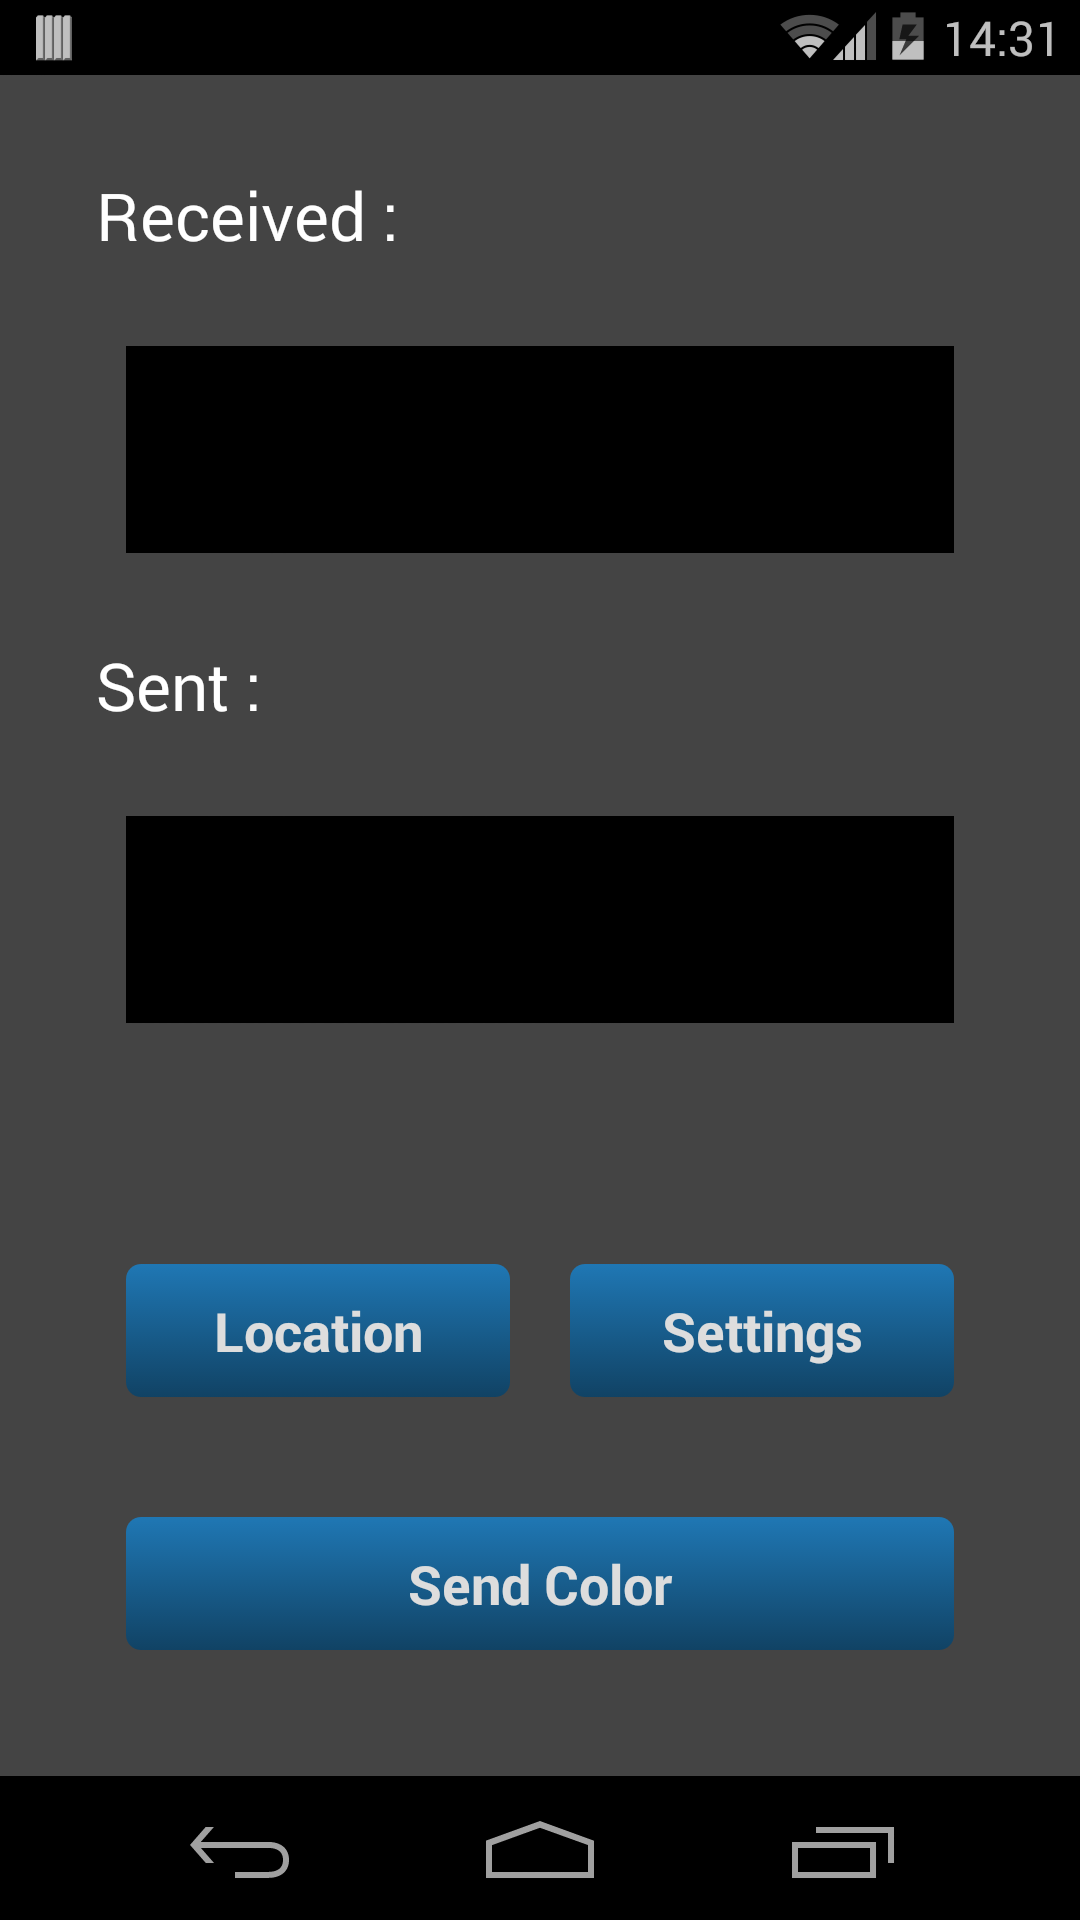
\includegraphics[width=4cm]{pictures/main.png}
	\caption{MainActivity layout}
	\label{fig:main}
\end{figure}




%----------------------------------------------------------------------------------------
%	SECTION
%----------------------------------------------------------------------------------------
\newpage
\section{Server implementation}
%----------------------------------------------------------------------------------------
\subsection{gcmserver.php}
\paragraph{}The server receives GET request with a parameter \verb?todo? that can take the value \verb?regid? for registration, \verb?colortoken? to send a nudge or \verb?locationtoken? to update location. Complementary arguments are sent using POST.



%----------------------------------------------------------------------------------------
\subsection{Database}

\paragraph{}
\begin{tabular}{rl}
name :& 'redblue' \\
host :& 'sql5.lri.fr' \\
user :& 'lfaucon' \\
password :& 'K4redblueSQL' \\
phpmyadmin :& '\verb?http://web-int.lri.fr/phpmyadmin/index.php?' \\
\end{tabular}

\paragraph{}The database contains two tables : \verb?user? and \verb?data?
\paragraph{Table user :}
\begin{tabular}{r|l}
name & name \\
regid & id for \textsc{Google cloud messaging} \\
login & login to link the couple \\
bffid & bff's id for \textsc{Google cloud messaging} \\
\end{tabular}
\paragraph{Table data :}
\begin{tabular}{r|l}
regid & id for \textsc{Google cloud messaging} \\
type & the type of the message : color or location \\
time & the time the message was sent (in milliseconds) \\
message & the content of the message \\
\end{tabular}

%----------------------------------------------------------------------------------------
\subsection{Data analysis}
\paragraph{}The file \verb?data.php? is a script to analyse the content of the database.


%----------------------------------------------------------------------------------------
%	BIBLIOGRAPHY
%----------------------------------------------------------------------------------------
\newpage
\section*{Références}
\paragraph{[1]}http://developer.android.com/
\paragraph{[2]}http://stackoverflow.com/



%----------------------------------------------------------------------------------------
\end{document}